\documentclass{beamer}
\usepackage[utf8]{inputenc}
\usepackage{fourier}

\usepackage{amsfonts}
\usepackage{amsmath}		
\usepackage{amssymb}
\usepackage{beamerthemesplit}
\usepackage{bezier}
\usepackage{float}
\usepackage{hyperref}
\usepackage{longtable}
\usepackage{makeidx}
\usepackage{rotating}
\usepackage{wrapfig}
\usepackage{multirow}
\usepackage{pgf}
\usepackage{ragged2e}

\usetheme{Madrid}
\usefonttheme{serif}
\usecolortheme{default}

\title[Graph Neural Networks]{Graph Neural Networks \\ Efficient Tensor Operations In CUDA/GPU \\ Custom Deep Learning Framework In C++ \\ Applications In Quantum Chemistry}
\author[Hy et al.]{Hy Truong Son, Chris Jones \\ Advisor: Prof. Risi Kondor}
\institute[UChicago]{The University of Chicago}
\date{December 2017}

\begin{document}

\logo{
\includegraphics[height=0.5cm]{Logo.jpg}}

\frame{\titlepage}

\begin{frame}
\frametitle{Table of Contents}
\tableofcontents
\end{frame}

\section{Chapter I: Introduction}

\begin{frame}
\frametitle{Our publication}
Covariant Compositional Networks For Learning Graphs (ICLR 2018)
\end{frame}

\begin{frame}
\frametitle{What are Graph Neural Networks?}
\begin{block}{Learning images, texts}
In general, traditional neural networks (Convolutional Neural Networks, Recurrent Neural Networks, etc.) take the inputs as \textbf{fixed-size} vectors, matrices and tensors. The architecture of the neural network is always \textbf{fixed}.
\end{block}
\begin{alertblock}{Learning graphs, molecules}
A graph neural network can be defined as a neural network that takes inputs from graphs with \textbf{various} sizes and structures. The architecture of the neural network is always \textbf{dynamic}.
\end{alertblock}
\end{frame}

\begin{frame}
\frametitle{What are Tensor Operations?}
Basic tensors:
\begin{itemize}
	\item 1D Tensor: Vectors
	\item 2D Tensor: Matrices
	\item 3D Tensor: Cubes
\end{itemize}
What we are dealing with: {\color{red} 6D Tensors}. We need the \textbf{tensor contraction} operation $C$ to reduce from the \textbf{high-order} into a \textbf{low-order}:
$$C: \Re^{d \times d \times d \times d \times d \times c} \rightarrow \Re^{d \times d \times c}$$
\end{frame}

\begin{frame}
\frametitle{What is GraphFlow framework?}
We write our own Deep Learning framework name {\color{red} GraphFlow} in C++ and CUDA to construct arbitrary neural networks that supports symbolic differentiation and dynamic computation graphs. 
\begin{itemize}
	\item Number of lines of C++ codes: $\sim 55,000$
	\item Total (including generated codes): $\sim 274,000$
	\item Done in this quarter for parallelization: {\color{red} $\sim 10,000$}
\end{itemize}
\end{frame}

\begin{frame}
\frametitle{Why not TensorFlow or PyTorch?}
\begin{block}{TensorFlow's disadvantage}
No (direct) support for dynamic computation graphs.
\end{block}
\begin{block}{PyTorch's disadvantage}
No support for tensor contractions.
\end{block}
\begin{alertblock}{GraphFlow's advantage}
	\begin{itemize}
		\item Support dynamic computation graphs
		\item Support tensor contractions
	\end{itemize}
\end{alertblock}
\end{frame}

\begin{frame}
\frametitle{Molecular Chemical Representation}
\begin{justify}
\begin{center}
	Harvard Clean Energy Project (HCEP) Dataset \cite{Johannes}
\end{center}
\begin{center}
	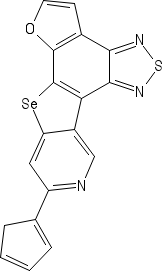
\includegraphics[scale=0.5]{sketcher}
\end{center}
Compound: C18H9N3OSSe \\
SMILES: C1C=CC=C1c1cc2[Se]c3c4occc4c4nsnc4c3c2cn1 \\
Power Conversion Efficiency (PCE, range 0 - 11): 5.16195
\end{justify}
\end{frame}

\begin{frame}
\frametitle{Molecular Graph Representation}
\begin{justify}
\begin{center}
	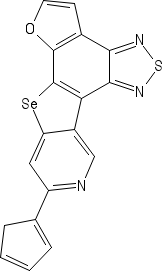
\includegraphics[scale=0.5]{sketcher}
	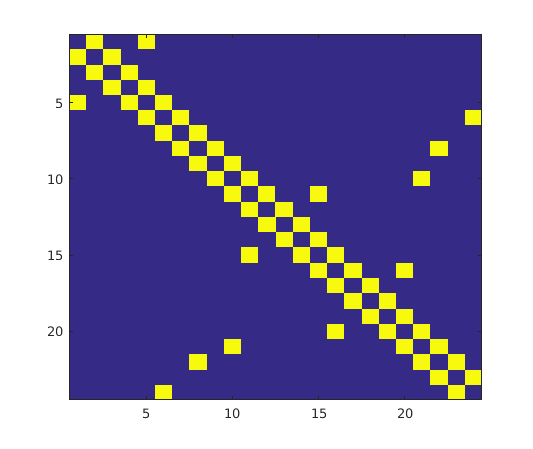
\includegraphics[scale=0.5]{adjacency}
\end{center}
C18H9N3OSSe \ \ \ \ \ \ \ \ \ \ \ \ \ \ \ \ \ \ \ \ Adjacency matrix
\end{justify}
\end{frame}

\section{Chapter II: State-of-the-art Algorithms}

\begin{frame}
\frametitle{Covariant (Graph) Neural Networks - Part 1}
Input graph $G = (V, E)$. Receptive field of vertex $v \in V$ at level $l = 0$ of the network: $\Omega_0(v) = \{v\}$. Receptive field of the vertex at level $l > 0$:
$$\Omega_l(v) = \Omega_{l - 1}(v) \cup \bigcup\limits_{w \in B(v, 1)} \Omega_{l - 1}(w)$$
High-order representation of vertex $v$ at level $l$:
$$f_l(v) \in \Re^{|\Omega_l(v)| \times |\Omega_l(v)| \times C}$$
where $C$ is the number of channels. We will learn the vertex representation by our graph neural networks with back-propagation. The representation has to be \textbf{permutation - invariant}.
\end{frame}

\begin{frame}
\frametitle{Covariant (Graph) Neural Networks - Part 2}
$$f_l(v) = \sigma \bigg( b_l + W_l \otimes \phi \bigg\{ \bigcup\limits_{w \in B(v, 1)} f_{l - 1}(w) \bigg\} \bigg)$$
where:
\begin{itemize}
	\item $\sigma$ is the Leaky ReLU activation function
	\item $b_l \in \Re^{1 \times 1 \times C}$ is the learnable bias
	\item $W_l \in \Re^{C \times (K \cdot C)}$ is the learnable weight matrix
	\item $C$ is the number of channels, $K$ is number of contractions
	\item $\otimes$ is the broad-casting matrix-tensor multiplication
	\item $f_{l - 1}(w) \in \Re^{|\Omega_{l - 1}(w)| \times |\Omega_{l - 1}(w)| \times C}$ is the vertex $w$ representation at level $l - 1$
	\item $\phi\{.\}$ is the combination of tensor product and tensor contraction operations of a set of high-order vertex representations
\end{itemize}
\end{frame}

\begin{frame}
\frametitle{Tensor Product and Tensor Contractions}
$$\phi \bigg\{ \bigcup\limits_{w \in B(v, 1)} f_{l - 1}(w) \bigg\}$$
can be expressed as:
\begin{itemize}
	\item We stack the set of 3D tensors $\{f_{l - 1}(w)\}$ into a 4D tensor $g_l(v)$
	\item We make the tensor product between $g_l(v)$ and the reduced adjacency matrix $A_{\Omega_l(v)}$ into a 6D tensor $h_l(v)$
	\item From the 6D tensor $h_l(v)$, we do the contraction to reduce to a 3D tensor $\phi_l(v)$
\end{itemize}
By combinatorics, there are exactly $K = 18$ unique ways of tensor contractions.
\end{frame}

\begin{frame}
\frametitle{Virtual Indexing System}
\begin{alertblock}{Huge tensor}
We cannot store a huge tensor $\Re^{|\Omega_l(v)| \times |\Omega_l(v)| \times |\Omega_l(v)| \times |\Omega_l(v)| \times |\Omega_l(v)| \times C}$ in memory explicitly.
\end{alertblock}
\begin{block}{Solution: Inspired from Virtual Machine}
We will not do the tensor product and tensor contraction directly, but via a \textbf{virtual indexing system} that allows us to access the value at position $(a, b, c, d, e, f)$ efficiently.
\end{block}
\end{frame}

\begin{frame}
\frametitle{GPU Multi-threading}
\end{frame}

\begin{frame}
\frametitle{CPU Multi-threading}
\end{frame}

\section{Chapter III: Experiments and Results}

\begin{frame}
\frametitle{Performance Test: GPU Matrix Multiplication}
\end{frame}

\begin{frame}
\frametitle{Performance Test: GPU Tensor Contractions}
\end{frame}

\begin{frame}
\frametitle{Small-scale Molecular Test}
\end{frame}

\begin{frame}
\frametitle{Real-world Dataset}
\end{frame}

\section{Chapter IV: Conclusion and Future Research}

\begin{frame}
\frametitle{Conclusion and Future Research}
\begin{justify}
We implemented the state-of-the-art generalized convolution operation for Graph Neural Networks in order to approximate Density Functional Theory. We obtained very promising results on the Harvard Clean Energy Project dataset.
$$$$
We are developing our custom Deep Learning framework in CUDA/C++ named \textbf{GraphFlow} which supports symbolic differentitation and dynamic computation graph. We expect that this framework will enable us to design more flexible, efficient Graph Neural Networks at a large scale in the future.
\end{justify}
\end{frame}

\begin{frame}
\frametitle{Acknowledgements}
\begin{justify}
We would like to acknowledge my advisor Professor Risi Kondor for his valuable instructions and especially for his great ideas in generalizing convolution operations in graphs. We also want to thank other members of Machine Learning group at the University of Chicago for their dedicated support.
$$$$
Some of the neural network training in this paper was done using the Midway cluster at the UChicago Computing Research Center.
\end{justify}
\end{frame}

\begin{frame}
\frametitle{Reference}
\begin{justify}
\begin{thebibliography}{9}

\bibitem[1]{Nino}
   N. Shervashidze, P. Schweitzer, E. J. van Leeuwen, K. Mehlhorn, K. M. Borgwardt,
   ``Weisfeiler-Lehman Graph Kernels'',
   \textit{Journal of Machine Learning Research}, vol.~12, 2011.
   
\bibitem[2]{Johannes}
   J. Hachmann, R. O. Amaya, S. A. Evrenk, C. A. Bedolla, R. S. S. Carrera, A. G. Parker, L. Vogt, A. M. Brockway, and A. A. Guzik,
   ``The Harvard Clean Energy Project: Large-Scale Computational Screening and Design of Organic Photovoltaics on the World Community Grid'',
   \textit{The Journal of Physical Chemistry Letters}, pp.~2241--2251, 2011.

\bibitem[3]{Risi}
   R. I. Kondor, and J. Lafferty,
   ``Diffusion Kernels on Graphs and Other Discrete Structures'',
   \textit{International Conference on Machine Learning (ICML)}, 2002.
   
\end{thebibliography}
\end{justify}
\end{frame}

\begin{frame}
\frametitle{Reference}
\begin{justify}
\begin{thebibliography}{9}

\bibitem[4]{Nils}
   N. M. Kriege, P. L. Giscard, R. C. Wilson,
   ``On Valid Optimal Assignment Kernels and Applications to Graph Classification'',
   \textit{Neural Information Processing Systems (NIPS)}, 2016.

\bibitem[5]{Steven}
   S. Kearnes, K. McCloskey, M. Berndl, V. Pande, P. Riley,
   ``Molecular Graph Convolutions: Moving Beyond Fingerprints'',
   \textit{Journal of Computer-Aided Molecular Design}, vol.~30, pp.~595--608, 2016.

\bibitem[6]{Duvenaud}
   D. Duvenaud, D. Maclaurin, J. A. Iparraguirre, R. G. Bombarelli, T. Hirzel, A. A. Guzik, R. P. Adams,
   ``Convolutional Networks on Graphs for Learning Molecular Fingerprints'',
   \textit{Neural Information Processing Systems (NIPS)}, 2015.
  
\end{thebibliography}
\end{justify}
\end{frame}

\begin{frame}
\frametitle{Reference}
\begin{justify}
\begin{thebibliography}{9}
   
\bibitem[7]{Thomas}
   T. N. Kipf, M. Welling,
   ``Semi-Supervised Classification with Graph Convolutional Networks'',
   \textit{International Conference on Learning Representations (ICLR)}, 2017.

\bibitem[8]{Maaten}
   L. V. D. Maaten, G. Hinton,
   ``Visualizing Data using t-SNE'',
   \textit{Journal of Machine Learning Research}, vol.~9, pp.~2579--2605, 2008.

\end{thebibliography}
\end{justify}
\end{frame}

\begin{frame}
\frametitle{}
\begin{center}
Thank you very much for your attention!
\end{center}
\end{frame}


\end{document}